\chapter{Theoretical Background} % Main chapter title
\label{chap:Chapter2} % For referencing the chapter elsewhere, use \ref{Chapter1} 
\epigraph{''Let no one ignorant of geometry enter” }{\textit{Plato}}

O χώρος των Wire
\begin{table}[H]
    \caption{Nodes' names definitions}
    \label{tab:drone-determined-by-their-structure}
    \centering
    \begin{tabular}{ll}
        \toprule
        \textbf{Node name} & \textbf{Definition}  \\
        \midrule
            Unknown/Free/Dumb/Non-anchors & Their position in unknown \\
			Beacons/Anchors/Landmarks & Nodes with known location information \\
			Settled & Unknown nodes that their position estimated \\
        \bottomrule
    \end{tabular}
\end{table}

\begin{figure} [H]
	\centering
	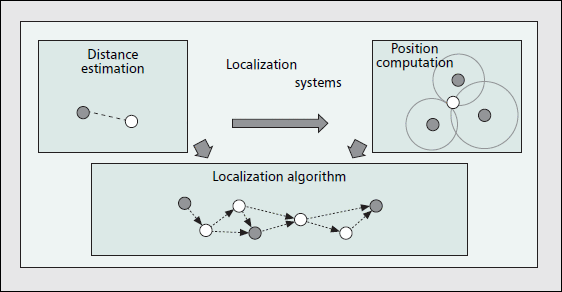
\includegraphics[scale=0.5]{Images/Theoretical-Background/localication-systems-components.png}
	\decoRule
	\caption[Localization Systems components]{Localization Systems components: \href{https://ieeexplore.ieee.org/document/4407221}{URL}}
	\label{fig:UAV-principal-axes}
\end{figure}

\tikzset{
  basic/.style  = {draw, text width=2cm, font=\sffamily},
  root/.style   = {basic, thin, align=center, fill=white, text width=5cm},
  level 1/.style = {sibling distance=16em, level distance=5em},
  level-2/.style = {basic, thin, align=center, fill=white, text width=5.5cm},
  level-31/.style = {basic, thin, align=center, fill=white, text width=2cm},
  level-32/.style = {basic, thin, align=center, fill=white, text width=2.8cm},
  level-33/.style = {basic, thin, align=center, fill=white, text width=5cm},
  level-4/.style = {basic, thin, align=center, fill=white, text width=4.5cm},
  level-42/.style = {basic, thin, align=center, fill=white, text width=4.8cm},
  edge from parent/.style={->,solid,black,thick,draw}, 
  edge from parent path={(\tikzparentnode.south) -- (\tikzchildnode.north)},
  >=latex, node distance=1.5cm, edge from parent fork down
}

\begin{figure} [H]
	\centering
	\resizebox{1\textwidth}{!}{
		\begin{tikzpicture}[]
			\node[root] {\textbf{Localization Systems}}
				child {node[level-2] (c1) {\textbf{Distance/Angle Estimation}}}
				child {node[level-2] (c2) {\textbf{Position Computation}}}
				child {node[level-2] (c3) {\textbf{Localization Algorithm}}};
			
			% -----------------------------------------------------------------------------
			% Distance/Angle
			\node [level-31, below of = c1, xshift=-25pt] (c11) {Distance};
				\node [level-4, below of = c11, xshift=50pt] (c111) {Received Signal Strength};
				\node [level-4, below of = c111] (c112) {Lighthouse};
				\node [level-4, below of = c112] (c113) {Propagation time based measurements};
					\node [level-42, below of = c113, xshift=30pt] (c1131) {One-way propagation time};
					\node [level-42, below of = c1131] (c1132) {Roundtrip propagation time};
					\node [level-42, below of = c1132] (c1133) {Time Difference of Arrival};
					\foreach \value in {1,2,3} \draw[->] (c113.197) |- (c113\value.west);
				\foreach \value in {1,2,3} \draw[->] (c11.195) |- (c11\value.west);

			\node [level-31, below of = c1133, xshift=-80pt] (c12) {Angle};
				\node [level-4, below of = c12, xshift=70pt] (c121) {Receiver Antenna Amplitude response};
				\node [level-4, below of = c121] (c122) {Receiver antenna Phase response};
				\foreach \value in {1,2} \draw[->] (c12.210) |- (c12\value.west);
			\foreach \value in {1,2}   \draw[->] (c1.188) |- (c1\value.west);
			
			% Position Computation
			\node [level-32, below of = c2, xshift=25pt] (c21) {Trilateration};
			\node [level-32, below of = c21] (c22) {Bounding box};
			\node [level-32, below of = c22] (c23) {Triangulation};
			\node [level-32, below of = c23] (c24) {Multilateration};
			\node [level-32, below of = c24] (c25) {Probabilistic approaches};
			\node [level-32, below of = c25] (c26) {Central position};
			\foreach \value in {1,...,6} \draw[->] (c2.196) |- (c2\value.west);

			% Localization Algorithm
			\node [level-33, below of = c3, xshift=10pt] (c31) {Distributed/Centralized \\ Position Computation};
			\node [level-33, below of = c31] (c32) {With/Without Infrastructure};
			\node [level-33, below of = c32] (c33) {Relative/Absolute Positioning};
			\node [level-33, below of = c33] (c34) {Indoor/Outdoor scenarios};
			\node [level-33, below of = c34] (c35) {One-hop/Multihop};
			\foreach \value in {1,...,5} \draw[->] (c3.187) |- (c3\value.west);
		\end{tikzpicture}
	}
	\decoRule
	\caption[Localization-system-overview]{Localization system overview}
	\label{fig:Localization-system}
\end{figure}
